% Created by tikzDevice version 0.12.6 on 2023-12-10 22:51:51
% !TEX encoding = UTF-8 Unicode
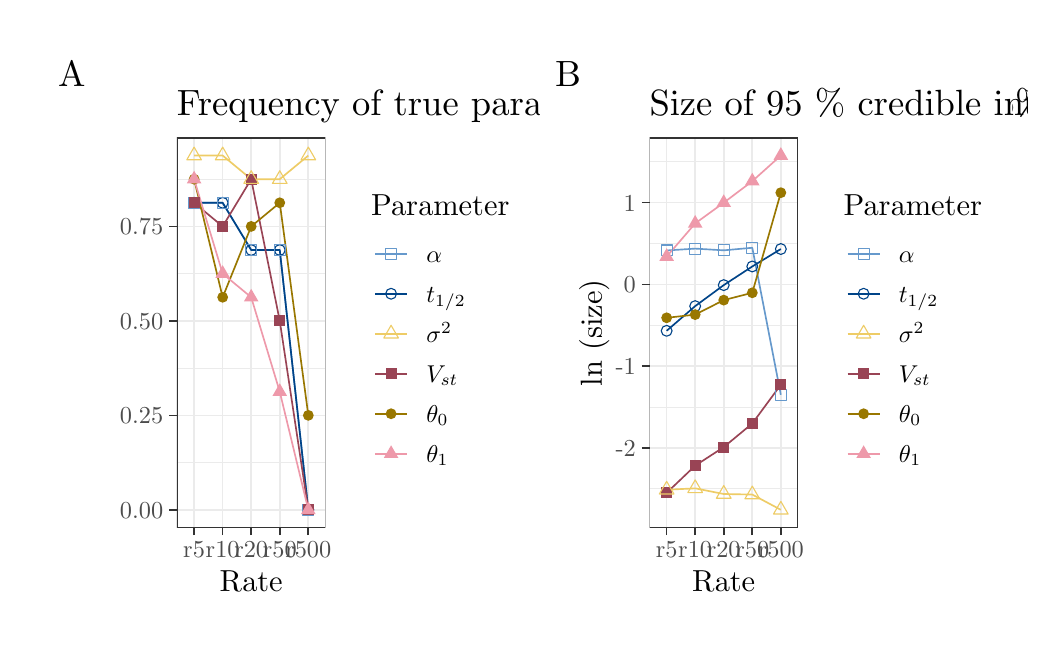
\begin{tikzpicture}[x=1pt,y=1pt]
\definecolor{fillColor}{RGB}{255,255,255}
\path[use as bounding box,fill=fillColor,fill opacity=0.00] (0,0) rectangle (361.35,216.81);
\begin{scope}
\path[clip] (  0.00,  0.00) rectangle (361.35,216.81);
\definecolor{drawColor}{RGB}{255,255,255}
\definecolor{fillColor}{RGB}{255,255,255}

\path[draw=drawColor,line width= 0.6pt,line join=round,line cap=round,fill=fillColor] (  0.00,  0.00) rectangle (361.35,216.81);
\end{scope}
\begin{scope}
\path[clip] (  5.50,  5.50) rectangle (185.10,211.31);
\definecolor{drawColor}{RGB}{255,255,255}
\definecolor{fillColor}{RGB}{255,255,255}

\path[draw=drawColor,line width= 0.6pt,line join=round,line cap=round,fill=fillColor] (  5.50,  5.50) rectangle (185.10,211.31);
\end{scope}
\begin{scope}
\path[clip] ( 53.95, 36.19) rectangle (107.60,177.00);
\definecolor{fillColor}{RGB}{255,255,255}

\path[fill=fillColor] ( 53.95, 36.19) rectangle (107.60,177.00);
\definecolor{drawColor}{gray}{0.92}

\path[draw=drawColor,line width= 0.3pt,line join=round] ( 53.95, 59.65) --
	(107.60, 59.65);

\path[draw=drawColor,line width= 0.3pt,line join=round] ( 53.95, 93.79) --
	(107.60, 93.79);

\path[draw=drawColor,line width= 0.3pt,line join=round] ( 53.95,127.93) --
	(107.60,127.93);

\path[draw=drawColor,line width= 0.3pt,line join=round] ( 53.95,162.06) --
	(107.60,162.06);

\path[draw=drawColor,line width= 0.6pt,line join=round] ( 53.95, 42.59) --
	(107.60, 42.59);

\path[draw=drawColor,line width= 0.6pt,line join=round] ( 53.95, 76.72) --
	(107.60, 76.72);

\path[draw=drawColor,line width= 0.6pt,line join=round] ( 53.95,110.86) --
	(107.60,110.86);

\path[draw=drawColor,line width= 0.6pt,line join=round] ( 53.95,144.99) --
	(107.60,144.99);

\path[draw=drawColor,line width= 0.6pt,line join=round] ( 60.14, 36.19) --
	( 60.14,177.00);

\path[draw=drawColor,line width= 0.6pt,line join=round] ( 70.46, 36.19) --
	( 70.46,177.00);

\path[draw=drawColor,line width= 0.6pt,line join=round] ( 80.77, 36.19) --
	( 80.77,177.00);

\path[draw=drawColor,line width= 0.6pt,line join=round] ( 91.09, 36.19) --
	( 91.09,177.00);

\path[draw=drawColor,line width= 0.6pt,line join=round] (101.41, 36.19) --
	(101.41,177.00);
\definecolor{drawColor}{RGB}{102,153,204}

\path[draw=drawColor,line width= 0.6pt,line join=round] ( 60.14,153.53) --
	( 70.46,153.53) --
	( 80.77,136.46) --
	( 91.09,136.46) --
	(101.41, 42.59);
\definecolor{drawColor}{RGB}{0,68,136}

\path[draw=drawColor,line width= 0.6pt,line join=round] ( 60.14,153.53) --
	( 70.46,153.53) --
	( 80.77,136.46) --
	( 91.09,136.46) --
	(101.41, 42.59);
\definecolor{drawColor}{RGB}{238,204,102}

\path[draw=drawColor,line width= 0.6pt,line join=round] ( 60.14,170.60) --
	( 70.46,170.60) --
	( 80.77,162.06) --
	( 91.09,162.06) --
	(101.41,170.60);
\definecolor{drawColor}{RGB}{153,68,85}

\path[draw=drawColor,line width= 0.6pt,line join=round] ( 60.14,153.53) --
	( 70.46,144.99) --
	( 80.77,162.06) --
	( 91.09,110.86) --
	(101.41, 42.59);
\definecolor{drawColor}{RGB}{153,119,0}

\path[draw=drawColor,line width= 0.6pt,line join=round] ( 60.14,162.06) --
	( 70.46,119.39) --
	( 80.77,144.99) --
	( 91.09,153.53) --
	(101.41, 76.72);
\definecolor{drawColor}{RGB}{238,153,170}

\path[draw=drawColor,line width= 0.6pt,line join=round] ( 60.14,162.06) --
	( 70.46,127.93) --
	( 80.77,119.39) --
	( 91.09, 85.26) --
	(101.41, 42.59);
\definecolor{drawColor}{RGB}{0,68,136}

\path[draw=drawColor,line width= 0.4pt,line join=round,line cap=round] ( 60.14,153.53) circle (  1.96);
\definecolor{drawColor}{RGB}{102,153,204}

\path[draw=drawColor,line width= 0.4pt,line join=round,line cap=round] ( 58.18,151.57) rectangle ( 62.10,155.49);
\definecolor{fillColor}{RGB}{153,68,85}

\path[fill=fillColor] ( 58.18,151.57) --
	( 62.10,151.57) --
	( 62.10,155.49) --
	( 58.18,155.49) --
	cycle;
\definecolor{drawColor}{RGB}{238,204,102}

\path[draw=drawColor,line width= 0.4pt,line join=round,line cap=round] ( 60.14,173.65) --
	( 62.78,169.07) --
	( 57.50,169.07) --
	cycle;
\definecolor{fillColor}{RGB}{153,119,0}

\path[fill=fillColor] ( 60.14,162.06) circle (  1.96);
\definecolor{fillColor}{RGB}{238,153,170}

\path[fill=fillColor] ( 60.14,165.11) --
	( 62.78,160.54) --
	( 57.50,160.54) --
	cycle;
\definecolor{drawColor}{RGB}{0,68,136}

\path[draw=drawColor,line width= 0.4pt,line join=round,line cap=round] ( 70.46,153.53) circle (  1.96);
\definecolor{drawColor}{RGB}{102,153,204}

\path[draw=drawColor,line width= 0.4pt,line join=round,line cap=round] ( 68.50,151.57) rectangle ( 72.42,155.49);
\definecolor{fillColor}{RGB}{153,68,85}

\path[fill=fillColor] ( 68.50,143.03) --
	( 72.42,143.03) --
	( 72.42,146.96) --
	( 68.50,146.96) --
	cycle;
\definecolor{drawColor}{RGB}{238,204,102}

\path[draw=drawColor,line width= 0.4pt,line join=round,line cap=round] ( 70.46,173.65) --
	( 73.10,169.07) --
	( 67.82,169.07) --
	cycle;
\definecolor{fillColor}{RGB}{153,119,0}

\path[fill=fillColor] ( 70.46,119.39) circle (  1.96);
\definecolor{fillColor}{RGB}{238,153,170}

\path[fill=fillColor] ( 70.46,130.98) --
	( 73.10,126.40) --
	( 67.82,126.40) --
	cycle;
\definecolor{drawColor}{RGB}{0,68,136}

\path[draw=drawColor,line width= 0.4pt,line join=round,line cap=round] ( 80.77,136.46) circle (  1.96);
\definecolor{drawColor}{RGB}{102,153,204}

\path[draw=drawColor,line width= 0.4pt,line join=round,line cap=round] ( 78.81,134.50) rectangle ( 82.74,138.42);
\definecolor{fillColor}{RGB}{153,68,85}

\path[fill=fillColor] ( 78.81,160.10) --
	( 82.74,160.10) --
	( 82.74,164.02) --
	( 78.81,164.02) --
	cycle;
\definecolor{drawColor}{RGB}{238,204,102}

\path[draw=drawColor,line width= 0.4pt,line join=round,line cap=round] ( 80.77,165.11) --
	( 83.42,160.54) --
	( 78.13,160.54) --
	cycle;
\definecolor{fillColor}{RGB}{153,119,0}

\path[fill=fillColor] ( 80.77,144.99) circle (  1.96);
\definecolor{fillColor}{RGB}{238,153,170}

\path[fill=fillColor] ( 80.77,122.44) --
	( 83.42,117.87) --
	( 78.13,117.87) --
	cycle;
\definecolor{drawColor}{RGB}{0,68,136}

\path[draw=drawColor,line width= 0.4pt,line join=round,line cap=round] ( 91.09,136.46) circle (  1.96);
\definecolor{drawColor}{RGB}{102,153,204}

\path[draw=drawColor,line width= 0.4pt,line join=round,line cap=round] ( 89.13,134.50) rectangle ( 93.05,138.42);
\definecolor{fillColor}{RGB}{153,68,85}

\path[fill=fillColor] ( 89.13,108.90) --
	( 93.05,108.90) --
	( 93.05,112.82) --
	( 89.13,112.82) --
	cycle;
\definecolor{drawColor}{RGB}{238,204,102}

\path[draw=drawColor,line width= 0.4pt,line join=round,line cap=round] ( 91.09,165.11) --
	( 93.73,160.54) --
	( 88.45,160.54) --
	cycle;
\definecolor{fillColor}{RGB}{153,119,0}

\path[fill=fillColor] ( 91.09,153.53) circle (  1.96);
\definecolor{fillColor}{RGB}{238,153,170}

\path[fill=fillColor] ( 91.09, 88.31) --
	( 93.73, 83.73) --
	( 88.45, 83.73) --
	cycle;
\definecolor{drawColor}{RGB}{0,68,136}

\path[draw=drawColor,line width= 0.4pt,line join=round,line cap=round] (101.41, 42.59) circle (  1.96);
\definecolor{drawColor}{RGB}{102,153,204}

\path[draw=drawColor,line width= 0.4pt,line join=round,line cap=round] ( 99.45, 40.62) rectangle (103.37, 44.55);
\definecolor{fillColor}{RGB}{153,68,85}

\path[fill=fillColor] ( 99.45, 40.62) --
	(103.37, 40.62) --
	(103.37, 44.55) --
	( 99.45, 44.55) --
	cycle;
\definecolor{drawColor}{RGB}{238,204,102}

\path[draw=drawColor,line width= 0.4pt,line join=round,line cap=round] (101.41,173.65) --
	(104.05,169.07) --
	( 98.76,169.07) --
	cycle;
\definecolor{fillColor}{RGB}{153,119,0}

\path[fill=fillColor] (101.41, 76.72) circle (  1.96);
\definecolor{fillColor}{RGB}{238,153,170}

\path[fill=fillColor] (101.41, 45.64) --
	(104.05, 41.06) --
	( 98.76, 41.06) --
	cycle;
\definecolor{drawColor}{gray}{0.20}

\path[draw=drawColor,line width= 0.6pt,line join=round,line cap=round] ( 53.95, 36.19) rectangle (107.60,177.00);
\end{scope}
\begin{scope}
\path[clip] (  0.00,  0.00) rectangle (361.35,216.81);
\definecolor{drawColor}{gray}{0.30}

\node[text=drawColor,anchor=base east,inner sep=0pt, outer sep=0pt, scale=  0.88] at ( 49.00, 39.56) {0.00};

\node[text=drawColor,anchor=base east,inner sep=0pt, outer sep=0pt, scale=  0.88] at ( 49.00, 73.69) {0.25};

\node[text=drawColor,anchor=base east,inner sep=0pt, outer sep=0pt, scale=  0.88] at ( 49.00,107.83) {0.50};

\node[text=drawColor,anchor=base east,inner sep=0pt, outer sep=0pt, scale=  0.88] at ( 49.00,141.96) {0.75};
\end{scope}
\begin{scope}
\path[clip] (  0.00,  0.00) rectangle (361.35,216.81);
\definecolor{drawColor}{gray}{0.20}

\path[draw=drawColor,line width= 0.6pt,line join=round] ( 51.20, 42.59) --
	( 53.95, 42.59);

\path[draw=drawColor,line width= 0.6pt,line join=round] ( 51.20, 76.72) --
	( 53.95, 76.72);

\path[draw=drawColor,line width= 0.6pt,line join=round] ( 51.20,110.86) --
	( 53.95,110.86);

\path[draw=drawColor,line width= 0.6pt,line join=round] ( 51.20,144.99) --
	( 53.95,144.99);
\end{scope}
\begin{scope}
\path[clip] (  0.00,  0.00) rectangle (361.35,216.81);
\definecolor{drawColor}{gray}{0.20}

\path[draw=drawColor,line width= 0.6pt,line join=round] ( 60.14, 33.44) --
	( 60.14, 36.19);

\path[draw=drawColor,line width= 0.6pt,line join=round] ( 70.46, 33.44) --
	( 70.46, 36.19);

\path[draw=drawColor,line width= 0.6pt,line join=round] ( 80.77, 33.44) --
	( 80.77, 36.19);

\path[draw=drawColor,line width= 0.6pt,line join=round] ( 91.09, 33.44) --
	( 91.09, 36.19);

\path[draw=drawColor,line width= 0.6pt,line join=round] (101.41, 33.44) --
	(101.41, 36.19);
\end{scope}
\begin{scope}
\path[clip] (  0.00,  0.00) rectangle (361.35,216.81);
\definecolor{drawColor}{gray}{0.30}

\node[text=drawColor,anchor=base,inner sep=0pt, outer sep=0pt, scale=  0.88] at ( 60.14, 25.18) {r5};

\node[text=drawColor,anchor=base,inner sep=0pt, outer sep=0pt, scale=  0.88] at ( 70.46, 25.18) {r10};

\node[text=drawColor,anchor=base,inner sep=0pt, outer sep=0pt, scale=  0.88] at ( 80.77, 25.18) {r20};

\node[text=drawColor,anchor=base,inner sep=0pt, outer sep=0pt, scale=  0.88] at ( 91.09, 25.18) {r50};

\node[text=drawColor,anchor=base,inner sep=0pt, outer sep=0pt, scale=  0.88] at (101.41, 25.18) {r500};
\end{scope}
\begin{scope}
\path[clip] (  0.00,  0.00) rectangle (361.35,216.81);
\definecolor{drawColor}{RGB}{0,0,0}

\node[text=drawColor,anchor=base,inner sep=0pt, outer sep=0pt, scale=  1.10] at ( 80.77, 13.14) {Rate};
\end{scope}
\begin{scope}
\path[clip] (  0.00,  0.00) rectangle (361.35,216.81);
\definecolor{fillColor}{RGB}{255,255,255}

\path[fill=fillColor] (118.60, 50.12) rectangle (179.60,163.06);
\end{scope}
\begin{scope}
\path[clip] (  0.00,  0.00) rectangle (361.35,216.81);
\definecolor{drawColor}{RGB}{0,0,0}

\node[text=drawColor,anchor=base west,inner sep=0pt, outer sep=0pt, scale=  1.10] at (124.10,148.91) {Parameter};
\end{scope}
\begin{scope}
\path[clip] (  0.00,  0.00) rectangle (361.35,216.81);
\definecolor{fillColor}{RGB}{255,255,255}

\path[fill=fillColor] (124.10,127.89) rectangle (138.55,142.35);
\end{scope}
\begin{scope}
\path[clip] (  0.00,  0.00) rectangle (361.35,216.81);
\definecolor{drawColor}{RGB}{102,153,204}

\path[draw=drawColor,line width= 0.6pt,line join=round] (125.54,135.12) -- (137.11,135.12);
\end{scope}
\begin{scope}
\path[clip] (  0.00,  0.00) rectangle (361.35,216.81);
\definecolor{drawColor}{RGB}{102,153,204}

\path[draw=drawColor,line width= 0.4pt,line join=round,line cap=round] (129.36,133.16) rectangle (133.29,137.08);
\end{scope}
\begin{scope}
\path[clip] (  0.00,  0.00) rectangle (361.35,216.81);
\definecolor{fillColor}{RGB}{255,255,255}

\path[fill=fillColor] (124.10,113.44) rectangle (138.55,127.89);
\end{scope}
\begin{scope}
\path[clip] (  0.00,  0.00) rectangle (361.35,216.81);
\definecolor{drawColor}{RGB}{0,68,136}

\path[draw=drawColor,line width= 0.6pt,line join=round] (125.54,120.66) -- (137.11,120.66);
\end{scope}
\begin{scope}
\path[clip] (  0.00,  0.00) rectangle (361.35,216.81);
\definecolor{drawColor}{RGB}{0,68,136}

\path[draw=drawColor,line width= 0.4pt,line join=round,line cap=round] (131.32,120.66) circle (  1.96);
\end{scope}
\begin{scope}
\path[clip] (  0.00,  0.00) rectangle (361.35,216.81);
\definecolor{fillColor}{RGB}{255,255,255}

\path[fill=fillColor] (124.10, 98.98) rectangle (138.55,113.44);
\end{scope}
\begin{scope}
\path[clip] (  0.00,  0.00) rectangle (361.35,216.81);
\definecolor{drawColor}{RGB}{238,204,102}

\path[draw=drawColor,line width= 0.6pt,line join=round] (125.54,106.21) -- (137.11,106.21);
\end{scope}
\begin{scope}
\path[clip] (  0.00,  0.00) rectangle (361.35,216.81);
\definecolor{drawColor}{RGB}{238,204,102}

\path[draw=drawColor,line width= 0.4pt,line join=round,line cap=round] (131.32,109.26) --
	(133.97,104.68) --
	(128.68,104.68) --
	cycle;
\end{scope}
\begin{scope}
\path[clip] (  0.00,  0.00) rectangle (361.35,216.81);
\definecolor{fillColor}{RGB}{255,255,255}

\path[fill=fillColor] (124.10, 84.53) rectangle (138.55, 98.98);
\end{scope}
\begin{scope}
\path[clip] (  0.00,  0.00) rectangle (361.35,216.81);
\definecolor{drawColor}{RGB}{153,68,85}

\path[draw=drawColor,line width= 0.6pt,line join=round] (125.54, 91.76) -- (137.11, 91.76);
\end{scope}
\begin{scope}
\path[clip] (  0.00,  0.00) rectangle (361.35,216.81);
\definecolor{fillColor}{RGB}{153,68,85}

\path[fill=fillColor] (129.36, 89.79) --
	(133.29, 89.79) --
	(133.29, 93.72) --
	(129.36, 93.72) --
	cycle;
\end{scope}
\begin{scope}
\path[clip] (  0.00,  0.00) rectangle (361.35,216.81);
\definecolor{fillColor}{RGB}{255,255,255}

\path[fill=fillColor] (124.10, 70.08) rectangle (138.55, 84.53);
\end{scope}
\begin{scope}
\path[clip] (  0.00,  0.00) rectangle (361.35,216.81);
\definecolor{drawColor}{RGB}{153,119,0}

\path[draw=drawColor,line width= 0.6pt,line join=round] (125.54, 77.30) -- (137.11, 77.30);
\end{scope}
\begin{scope}
\path[clip] (  0.00,  0.00) rectangle (361.35,216.81);
\definecolor{fillColor}{RGB}{153,119,0}

\path[fill=fillColor] (131.32, 77.30) circle (  1.96);
\end{scope}
\begin{scope}
\path[clip] (  0.00,  0.00) rectangle (361.35,216.81);
\definecolor{fillColor}{RGB}{255,255,255}

\path[fill=fillColor] (124.10, 55.62) rectangle (138.55, 70.08);
\end{scope}
\begin{scope}
\path[clip] (  0.00,  0.00) rectangle (361.35,216.81);
\definecolor{drawColor}{RGB}{238,153,170}

\path[draw=drawColor,line width= 0.6pt,line join=round] (125.54, 62.85) -- (137.11, 62.85);
\end{scope}
\begin{scope}
\path[clip] (  0.00,  0.00) rectangle (361.35,216.81);
\definecolor{fillColor}{RGB}{238,153,170}

\path[fill=fillColor] (131.32, 65.90) --
	(133.97, 61.32) --
	(128.68, 61.32) --
	cycle;
\end{scope}
\begin{scope}
\path[clip] (  0.00,  0.00) rectangle (361.35,216.81);
\definecolor{drawColor}{RGB}{0,0,0}

\node[text=drawColor,anchor=base west,inner sep=0pt, outer sep=0pt, scale=  0.88] at (144.05,132.09) {$\alpha$};
\end{scope}
\begin{scope}
\path[clip] (  0.00,  0.00) rectangle (361.35,216.81);
\definecolor{drawColor}{RGB}{0,0,0}

\node[text=drawColor,anchor=base west,inner sep=0pt, outer sep=0pt, scale=  0.88] at (144.05,117.63) {$t_{1/2}$};
\end{scope}
\begin{scope}
\path[clip] (  0.00,  0.00) rectangle (361.35,216.81);
\definecolor{drawColor}{RGB}{0,0,0}

\node[text=drawColor,anchor=base west,inner sep=0pt, outer sep=0pt, scale=  0.88] at (144.05,103.18) {$\sigma^2$};
\end{scope}
\begin{scope}
\path[clip] (  0.00,  0.00) rectangle (361.35,216.81);
\definecolor{drawColor}{RGB}{0,0,0}

\node[text=drawColor,anchor=base west,inner sep=0pt, outer sep=0pt, scale=  0.88] at (144.05, 88.73) {$V_{st}$};
\end{scope}
\begin{scope}
\path[clip] (  0.00,  0.00) rectangle (361.35,216.81);
\definecolor{drawColor}{RGB}{0,0,0}

\node[text=drawColor,anchor=base west,inner sep=0pt, outer sep=0pt, scale=  0.88] at (144.05, 74.27) {$\theta_0$};
\end{scope}
\begin{scope}
\path[clip] (  0.00,  0.00) rectangle (361.35,216.81);
\definecolor{drawColor}{RGB}{0,0,0}

\node[text=drawColor,anchor=base west,inner sep=0pt, outer sep=0pt, scale=  0.88] at (144.05, 59.82) {$\theta_1$};
\end{scope}
\begin{scope}
\path[clip] (  0.00,  0.00) rectangle (361.35,216.81);
\definecolor{drawColor}{RGB}{0,0,0}

\node[text=drawColor,anchor=base west,inner sep=0pt, outer sep=0pt, scale=  1.32] at ( 53.95,185.06) {Frequency of true parameter values falling within  $\newline 95\%$ credible interval};
\end{scope}
\begin{scope}
\path[clip] (  0.00,  0.00) rectangle (361.35,216.81);
\definecolor{drawColor}{RGB}{0,0,0}

\node[text=drawColor,anchor=base,inner sep=0pt, outer sep=0pt, scale=  1.32] at ( 15.95,195.44) {A};
\end{scope}
\begin{scope}
\path[clip] (185.10,  5.50) rectangle (355.85,211.31);
\definecolor{drawColor}{RGB}{255,255,255}
\definecolor{fillColor}{RGB}{255,255,255}

\path[draw=drawColor,line width= 0.6pt,line join=round,line cap=round,fill=fillColor] (185.10,  5.50) rectangle (355.85,211.31);
\end{scope}
\begin{scope}
\path[clip] (224.70, 36.19) rectangle (278.34,177.00);
\definecolor{fillColor}{RGB}{255,255,255}

\path[fill=fillColor] (224.70, 36.19) rectangle (278.34,177.00);
\definecolor{drawColor}{gray}{0.92}

\path[draw=drawColor,line width= 0.3pt,line join=round] (224.70, 50.22) --
	(278.34, 50.22);

\path[draw=drawColor,line width= 0.3pt,line join=round] (224.70, 79.75) --
	(278.34, 79.75);

\path[draw=drawColor,line width= 0.3pt,line join=round] (224.70,109.29) --
	(278.34,109.29);

\path[draw=drawColor,line width= 0.3pt,line join=round] (224.70,138.82) --
	(278.34,138.82);

\path[draw=drawColor,line width= 0.3pt,line join=round] (224.70,168.36) --
	(278.34,168.36);

\path[draw=drawColor,line width= 0.6pt,line join=round] (224.70, 64.98) --
	(278.34, 64.98);

\path[draw=drawColor,line width= 0.6pt,line join=round] (224.70, 94.52) --
	(278.34, 94.52);

\path[draw=drawColor,line width= 0.6pt,line join=round] (224.70,124.06) --
	(278.34,124.06);

\path[draw=drawColor,line width= 0.6pt,line join=round] (224.70,153.59) --
	(278.34,153.59);

\path[draw=drawColor,line width= 0.6pt,line join=round] (230.89, 36.19) --
	(230.89,177.00);

\path[draw=drawColor,line width= 0.6pt,line join=round] (241.20, 36.19) --
	(241.20,177.00);

\path[draw=drawColor,line width= 0.6pt,line join=round] (251.52, 36.19) --
	(251.52,177.00);

\path[draw=drawColor,line width= 0.6pt,line join=round] (261.84, 36.19) --
	(261.84,177.00);

\path[draw=drawColor,line width= 0.6pt,line join=round] (272.15, 36.19) --
	(272.15,177.00);
\definecolor{drawColor}{RGB}{102,153,204}

\path[draw=drawColor,line width= 0.6pt,line join=round] (230.89,136.30) --
	(241.20,136.97) --
	(251.52,136.35) --
	(261.84,137.28) --
	(272.15, 84.17);
\definecolor{drawColor}{RGB}{0,68,136}

\path[draw=drawColor,line width= 0.6pt,line join=round] (230.89,107.27) --
	(241.20,116.19) --
	(251.52,123.78) --
	(261.84,130.52) --
	(272.15,136.82);
\definecolor{drawColor}{RGB}{238,204,102}

\path[draw=drawColor,line width= 0.6pt,line join=round] (230.89, 49.83) --
	(241.20, 50.35) --
	(251.52, 48.30) --
	(261.84, 48.10) --
	(272.15, 42.59);
\definecolor{drawColor}{RGB}{153,68,85}

\path[draw=drawColor,line width= 0.6pt,line join=round] (230.89, 48.71) --
	(241.20, 58.54) --
	(251.52, 65.24) --
	(261.84, 73.78) --
	(272.15, 87.79);
\definecolor{drawColor}{RGB}{153,119,0}

\path[draw=drawColor,line width= 0.6pt,line join=round] (230.89,111.97) --
	(241.20,113.12) --
	(251.52,118.36) --
	(261.84,121.01) --
	(272.15,157.18);
\definecolor{drawColor}{RGB}{238,153,170}

\path[draw=drawColor,line width= 0.6pt,line join=round] (230.89,134.07) --
	(241.20,146.07) --
	(251.52,153.56) --
	(261.84,161.34) --
	(272.15,170.60);
\definecolor{drawColor}{RGB}{0,68,136}

\path[draw=drawColor,line width= 0.4pt,line join=round,line cap=round] (230.89,107.27) circle (  1.96);
\definecolor{drawColor}{RGB}{102,153,204}

\path[draw=drawColor,line width= 0.4pt,line join=round,line cap=round] (228.93,134.33) rectangle (232.85,138.26);
\definecolor{fillColor}{RGB}{153,68,85}

\path[fill=fillColor] (228.93, 46.75) --
	(232.85, 46.75) --
	(232.85, 50.68) --
	(228.93, 50.68) --
	cycle;
\definecolor{drawColor}{RGB}{238,204,102}

\path[draw=drawColor,line width= 0.4pt,line join=round,line cap=round] (230.89, 52.88) --
	(233.53, 48.31) --
	(228.25, 48.31) --
	cycle;
\definecolor{fillColor}{RGB}{153,119,0}

\path[fill=fillColor] (230.89,111.97) circle (  1.96);
\definecolor{fillColor}{RGB}{238,153,170}

\path[fill=fillColor] (230.89,137.12) --
	(233.53,132.55) --
	(228.25,132.55) --
	cycle;
\definecolor{drawColor}{RGB}{0,68,136}

\path[draw=drawColor,line width= 0.4pt,line join=round,line cap=round] (241.20,116.19) circle (  1.96);
\definecolor{drawColor}{RGB}{102,153,204}

\path[draw=drawColor,line width= 0.4pt,line join=round,line cap=round] (239.24,135.00) rectangle (243.17,138.93);
\definecolor{fillColor}{RGB}{153,68,85}

\path[fill=fillColor] (239.24, 56.58) --
	(243.17, 56.58) --
	(243.17, 60.51) --
	(239.24, 60.51) --
	cycle;
\definecolor{drawColor}{RGB}{238,204,102}

\path[draw=drawColor,line width= 0.4pt,line join=round,line cap=round] (241.20, 53.40) --
	(243.85, 48.82) --
	(238.56, 48.82) --
	cycle;
\definecolor{fillColor}{RGB}{153,119,0}

\path[fill=fillColor] (241.20,113.12) circle (  1.96);
\definecolor{fillColor}{RGB}{238,153,170}

\path[fill=fillColor] (241.20,149.12) --
	(243.85,144.54) --
	(238.56,144.54) --
	cycle;
\definecolor{drawColor}{RGB}{0,68,136}

\path[draw=drawColor,line width= 0.4pt,line join=round,line cap=round] (251.52,123.78) circle (  1.96);
\definecolor{drawColor}{RGB}{102,153,204}

\path[draw=drawColor,line width= 0.4pt,line join=round,line cap=round] (249.56,134.38) rectangle (253.48,138.31);
\definecolor{fillColor}{RGB}{153,68,85}

\path[fill=fillColor] (249.56, 63.28) --
	(253.48, 63.28) --
	(253.48, 67.20) --
	(249.56, 67.20) --
	cycle;
\definecolor{drawColor}{RGB}{238,204,102}

\path[draw=drawColor,line width= 0.4pt,line join=round,line cap=round] (251.52, 51.36) --
	(254.16, 46.78) --
	(248.88, 46.78) --
	cycle;
\definecolor{fillColor}{RGB}{153,119,0}

\path[fill=fillColor] (251.52,118.36) circle (  1.96);
\definecolor{fillColor}{RGB}{238,153,170}

\path[fill=fillColor] (251.52,156.61) --
	(254.16,152.03) --
	(248.88,152.03) --
	cycle;
\definecolor{drawColor}{RGB}{0,68,136}

\path[draw=drawColor,line width= 0.4pt,line join=round,line cap=round] (261.84,130.52) circle (  1.96);
\definecolor{drawColor}{RGB}{102,153,204}

\path[draw=drawColor,line width= 0.4pt,line join=round,line cap=round] (259.87,135.32) rectangle (263.80,139.24);
\definecolor{fillColor}{RGB}{153,68,85}

\path[fill=fillColor] (259.87, 71.82) --
	(263.80, 71.82) --
	(263.80, 75.74) --
	(259.87, 75.74) --
	cycle;
\definecolor{drawColor}{RGB}{238,204,102}

\path[draw=drawColor,line width= 0.4pt,line join=round,line cap=round] (261.84, 51.15) --
	(264.48, 46.58) --
	(259.19, 46.58) --
	cycle;
\definecolor{fillColor}{RGB}{153,119,0}

\path[fill=fillColor] (261.84,121.01) circle (  1.96);
\definecolor{fillColor}{RGB}{238,153,170}

\path[fill=fillColor] (261.84,164.39) --
	(264.48,159.81) --
	(259.19,159.81) --
	cycle;
\definecolor{drawColor}{RGB}{0,68,136}

\path[draw=drawColor,line width= 0.4pt,line join=round,line cap=round] (272.15,136.82) circle (  1.96);
\definecolor{drawColor}{RGB}{102,153,204}

\path[draw=drawColor,line width= 0.4pt,line join=round,line cap=round] (270.19, 82.20) rectangle (274.11, 86.13);
\definecolor{fillColor}{RGB}{153,68,85}

\path[fill=fillColor] (270.19, 85.82) --
	(274.11, 85.82) --
	(274.11, 89.75) --
	(270.19, 89.75) --
	cycle;
\definecolor{drawColor}{RGB}{238,204,102}

\path[draw=drawColor,line width= 0.4pt,line join=round,line cap=round] (272.15, 45.64) --
	(274.80, 41.06) --
	(269.51, 41.06) --
	cycle;
\definecolor{fillColor}{RGB}{153,119,0}

\path[fill=fillColor] (272.15,157.18) circle (  1.96);
\definecolor{fillColor}{RGB}{238,153,170}

\path[fill=fillColor] (272.15,173.65) --
	(274.80,169.07) --
	(269.51,169.07) --
	cycle;
\definecolor{drawColor}{gray}{0.20}

\path[draw=drawColor,line width= 0.6pt,line join=round,line cap=round] (224.70, 36.19) rectangle (278.34,177.00);
\end{scope}
\begin{scope}
\path[clip] (  0.00,  0.00) rectangle (361.35,216.81);
\definecolor{drawColor}{gray}{0.30}

\node[text=drawColor,anchor=base east,inner sep=0pt, outer sep=0pt, scale=  0.88] at (219.75, 61.95) {-2};

\node[text=drawColor,anchor=base east,inner sep=0pt, outer sep=0pt, scale=  0.88] at (219.75, 91.49) {-1};

\node[text=drawColor,anchor=base east,inner sep=0pt, outer sep=0pt, scale=  0.88] at (219.75,121.03) {0};

\node[text=drawColor,anchor=base east,inner sep=0pt, outer sep=0pt, scale=  0.88] at (219.75,150.56) {1};
\end{scope}
\begin{scope}
\path[clip] (  0.00,  0.00) rectangle (361.35,216.81);
\definecolor{drawColor}{gray}{0.20}

\path[draw=drawColor,line width= 0.6pt,line join=round] (221.95, 64.98) --
	(224.70, 64.98);

\path[draw=drawColor,line width= 0.6pt,line join=round] (221.95, 94.52) --
	(224.70, 94.52);

\path[draw=drawColor,line width= 0.6pt,line join=round] (221.95,124.06) --
	(224.70,124.06);

\path[draw=drawColor,line width= 0.6pt,line join=round] (221.95,153.59) --
	(224.70,153.59);
\end{scope}
\begin{scope}
\path[clip] (  0.00,  0.00) rectangle (361.35,216.81);
\definecolor{drawColor}{gray}{0.20}

\path[draw=drawColor,line width= 0.6pt,line join=round] (230.89, 33.44) --
	(230.89, 36.19);

\path[draw=drawColor,line width= 0.6pt,line join=round] (241.20, 33.44) --
	(241.20, 36.19);

\path[draw=drawColor,line width= 0.6pt,line join=round] (251.52, 33.44) --
	(251.52, 36.19);

\path[draw=drawColor,line width= 0.6pt,line join=round] (261.84, 33.44) --
	(261.84, 36.19);

\path[draw=drawColor,line width= 0.6pt,line join=round] (272.15, 33.44) --
	(272.15, 36.19);
\end{scope}
\begin{scope}
\path[clip] (  0.00,  0.00) rectangle (361.35,216.81);
\definecolor{drawColor}{gray}{0.30}

\node[text=drawColor,anchor=base,inner sep=0pt, outer sep=0pt, scale=  0.88] at (230.89, 25.18) {r5};

\node[text=drawColor,anchor=base,inner sep=0pt, outer sep=0pt, scale=  0.88] at (241.20, 25.18) {r10};

\node[text=drawColor,anchor=base,inner sep=0pt, outer sep=0pt, scale=  0.88] at (251.52, 25.18) {r20};

\node[text=drawColor,anchor=base,inner sep=0pt, outer sep=0pt, scale=  0.88] at (261.84, 25.18) {r50};

\node[text=drawColor,anchor=base,inner sep=0pt, outer sep=0pt, scale=  0.88] at (272.15, 25.18) {r500};
\end{scope}
\begin{scope}
\path[clip] (  0.00,  0.00) rectangle (361.35,216.81);
\definecolor{drawColor}{RGB}{0,0,0}

\node[text=drawColor,anchor=base,inner sep=0pt, outer sep=0pt, scale=  1.10] at (251.52, 13.14) {Rate};
\end{scope}
\begin{scope}
\path[clip] (  0.00,  0.00) rectangle (361.35,216.81);
\definecolor{drawColor}{RGB}{0,0,0}

\node[text=drawColor,rotate= 90.00,anchor=base,inner sep=0pt, outer sep=0pt, scale=  1.10] at (207.53,106.59) {$\ln$ (size)};
\end{scope}
\begin{scope}
\path[clip] (  0.00,  0.00) rectangle (361.35,216.81);
\definecolor{fillColor}{RGB}{255,255,255}

\path[fill=fillColor] (289.34, 50.12) rectangle (350.35,163.06);
\end{scope}
\begin{scope}
\path[clip] (  0.00,  0.00) rectangle (361.35,216.81);
\definecolor{drawColor}{RGB}{0,0,0}

\node[text=drawColor,anchor=base west,inner sep=0pt, outer sep=0pt, scale=  1.10] at (294.84,148.91) {Parameter};
\end{scope}
\begin{scope}
\path[clip] (  0.00,  0.00) rectangle (361.35,216.81);
\definecolor{fillColor}{RGB}{255,255,255}

\path[fill=fillColor] (294.84,127.89) rectangle (309.30,142.35);
\end{scope}
\begin{scope}
\path[clip] (  0.00,  0.00) rectangle (361.35,216.81);
\definecolor{drawColor}{RGB}{102,153,204}

\path[draw=drawColor,line width= 0.6pt,line join=round] (296.29,135.12) -- (307.85,135.12);
\end{scope}
\begin{scope}
\path[clip] (  0.00,  0.00) rectangle (361.35,216.81);
\definecolor{drawColor}{RGB}{102,153,204}

\path[draw=drawColor,line width= 0.4pt,line join=round,line cap=round] (300.11,133.16) rectangle (304.03,137.08);
\end{scope}
\begin{scope}
\path[clip] (  0.00,  0.00) rectangle (361.35,216.81);
\definecolor{fillColor}{RGB}{255,255,255}

\path[fill=fillColor] (294.84,113.44) rectangle (309.30,127.89);
\end{scope}
\begin{scope}
\path[clip] (  0.00,  0.00) rectangle (361.35,216.81);
\definecolor{drawColor}{RGB}{0,68,136}

\path[draw=drawColor,line width= 0.6pt,line join=round] (296.29,120.66) -- (307.85,120.66);
\end{scope}
\begin{scope}
\path[clip] (  0.00,  0.00) rectangle (361.35,216.81);
\definecolor{drawColor}{RGB}{0,68,136}

\path[draw=drawColor,line width= 0.4pt,line join=round,line cap=round] (302.07,120.66) circle (  1.96);
\end{scope}
\begin{scope}
\path[clip] (  0.00,  0.00) rectangle (361.35,216.81);
\definecolor{fillColor}{RGB}{255,255,255}

\path[fill=fillColor] (294.84, 98.98) rectangle (309.30,113.44);
\end{scope}
\begin{scope}
\path[clip] (  0.00,  0.00) rectangle (361.35,216.81);
\definecolor{drawColor}{RGB}{238,204,102}

\path[draw=drawColor,line width= 0.6pt,line join=round] (296.29,106.21) -- (307.85,106.21);
\end{scope}
\begin{scope}
\path[clip] (  0.00,  0.00) rectangle (361.35,216.81);
\definecolor{drawColor}{RGB}{238,204,102}

\path[draw=drawColor,line width= 0.4pt,line join=round,line cap=round] (302.07,109.26) --
	(304.71,104.68) --
	(299.43,104.68) --
	cycle;
\end{scope}
\begin{scope}
\path[clip] (  0.00,  0.00) rectangle (361.35,216.81);
\definecolor{fillColor}{RGB}{255,255,255}

\path[fill=fillColor] (294.84, 84.53) rectangle (309.30, 98.98);
\end{scope}
\begin{scope}
\path[clip] (  0.00,  0.00) rectangle (361.35,216.81);
\definecolor{drawColor}{RGB}{153,68,85}

\path[draw=drawColor,line width= 0.6pt,line join=round] (296.29, 91.76) -- (307.85, 91.76);
\end{scope}
\begin{scope}
\path[clip] (  0.00,  0.00) rectangle (361.35,216.81);
\definecolor{fillColor}{RGB}{153,68,85}

\path[fill=fillColor] (300.11, 89.79) --
	(304.03, 89.79) --
	(304.03, 93.72) --
	(300.11, 93.72) --
	cycle;
\end{scope}
\begin{scope}
\path[clip] (  0.00,  0.00) rectangle (361.35,216.81);
\definecolor{fillColor}{RGB}{255,255,255}

\path[fill=fillColor] (294.84, 70.08) rectangle (309.30, 84.53);
\end{scope}
\begin{scope}
\path[clip] (  0.00,  0.00) rectangle (361.35,216.81);
\definecolor{drawColor}{RGB}{153,119,0}

\path[draw=drawColor,line width= 0.6pt,line join=round] (296.29, 77.30) -- (307.85, 77.30);
\end{scope}
\begin{scope}
\path[clip] (  0.00,  0.00) rectangle (361.35,216.81);
\definecolor{fillColor}{RGB}{153,119,0}

\path[fill=fillColor] (302.07, 77.30) circle (  1.96);
\end{scope}
\begin{scope}
\path[clip] (  0.00,  0.00) rectangle (361.35,216.81);
\definecolor{fillColor}{RGB}{255,255,255}

\path[fill=fillColor] (294.84, 55.62) rectangle (309.30, 70.08);
\end{scope}
\begin{scope}
\path[clip] (  0.00,  0.00) rectangle (361.35,216.81);
\definecolor{drawColor}{RGB}{238,153,170}

\path[draw=drawColor,line width= 0.6pt,line join=round] (296.29, 62.85) -- (307.85, 62.85);
\end{scope}
\begin{scope}
\path[clip] (  0.00,  0.00) rectangle (361.35,216.81);
\definecolor{fillColor}{RGB}{238,153,170}

\path[fill=fillColor] (302.07, 65.90) --
	(304.71, 61.32) --
	(299.43, 61.32) --
	cycle;
\end{scope}
\begin{scope}
\path[clip] (  0.00,  0.00) rectangle (361.35,216.81);
\definecolor{drawColor}{RGB}{0,0,0}

\node[text=drawColor,anchor=base west,inner sep=0pt, outer sep=0pt, scale=  0.88] at (314.80,132.09) {$\alpha$};
\end{scope}
\begin{scope}
\path[clip] (  0.00,  0.00) rectangle (361.35,216.81);
\definecolor{drawColor}{RGB}{0,0,0}

\node[text=drawColor,anchor=base west,inner sep=0pt, outer sep=0pt, scale=  0.88] at (314.80,117.63) {$t_{1/2}$};
\end{scope}
\begin{scope}
\path[clip] (  0.00,  0.00) rectangle (361.35,216.81);
\definecolor{drawColor}{RGB}{0,0,0}

\node[text=drawColor,anchor=base west,inner sep=0pt, outer sep=0pt, scale=  0.88] at (314.80,103.18) {$\sigma^2$};
\end{scope}
\begin{scope}
\path[clip] (  0.00,  0.00) rectangle (361.35,216.81);
\definecolor{drawColor}{RGB}{0,0,0}

\node[text=drawColor,anchor=base west,inner sep=0pt, outer sep=0pt, scale=  0.88] at (314.80, 88.73) {$V_{st}$};
\end{scope}
\begin{scope}
\path[clip] (  0.00,  0.00) rectangle (361.35,216.81);
\definecolor{drawColor}{RGB}{0,0,0}

\node[text=drawColor,anchor=base west,inner sep=0pt, outer sep=0pt, scale=  0.88] at (314.80, 74.27) {$\theta_0$};
\end{scope}
\begin{scope}
\path[clip] (  0.00,  0.00) rectangle (361.35,216.81);
\definecolor{drawColor}{RGB}{0,0,0}

\node[text=drawColor,anchor=base west,inner sep=0pt, outer sep=0pt, scale=  0.88] at (314.80, 59.82) {$\theta_1$};
\end{scope}
\begin{scope}
\path[clip] (  0.00,  0.00) rectangle (361.35,216.81);
\definecolor{drawColor}{RGB}{0,0,0}

\node[text=drawColor,anchor=base west,inner sep=0pt, outer sep=0pt, scale=  1.32] at (224.70,185.06) {Size of 95 $\%$ credible interval};
\end{scope}
\begin{scope}
\path[clip] (  0.00,  0.00) rectangle (361.35,216.81);
\definecolor{drawColor}{RGB}{0,0,0}

\node[text=drawColor,anchor=base,inner sep=0pt, outer sep=0pt, scale=  1.32] at (195.28,195.44) {B};
\end{scope}
\end{tikzpicture}
